\documentclass{article}
\usepackage[utf8]{inputenc}
\usepackage{graphicx}
\usepackage{geometry}
\geometry{a4paper, margin=1in}
\usepackage{hyperref}

\title{Programming Assignment 2: Report}
\author{Jai Shanakr Azad \\ M25CSA014}
\date{March 20, 2026}

\begin{document}

\maketitle

\section*{PROBLEM 1: LEARNING WORD EMBEDDINGS FROM IIT JODHPUR DATA}

\subsection*{TASK 1: DATASET PREPARATION}

To collect the dataset, I scraped several official pages from the IIT Jodhpur website, including the main page, academic programs, department structures, research page, and the student's office page. The scraped content was processed by removing boilerplate text, tokenization, lowercasing, and removing non-textual tokens like URLs and punctuation.

\textbf{Dataset Statistics:}
\begin{itemize}
    \item \textbf{Total number of documents (sentences):} 5203
    \item \textbf{Total number of tokens:} 142,555
    \item \textbf{Vocabulary size:} 2,393
    \item \textbf{Average tokens per document:} 27.4
\end{itemize}

\textbf{Word Cloud of Most Frequent Words:}

\begin{figure}[htbp]
    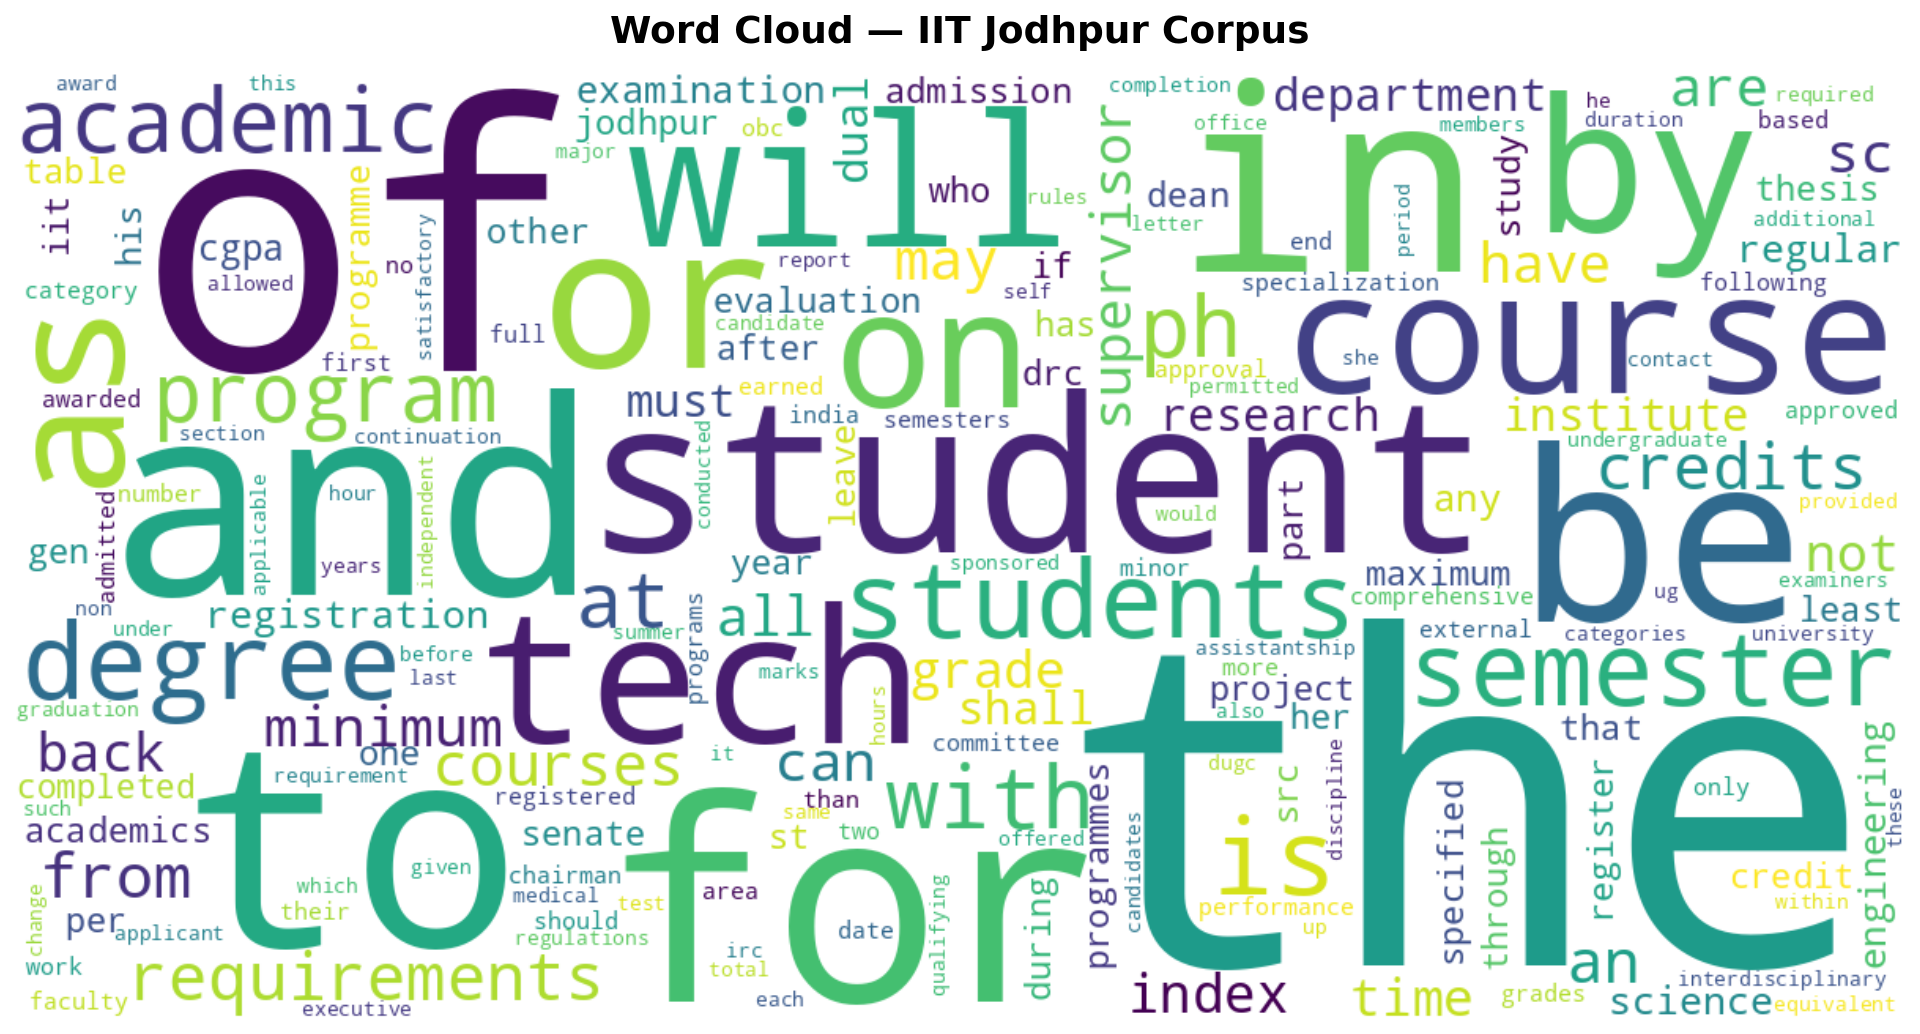
\includegraphics[width=0.8\textwidth]{wordcloud.png}
    \caption{Word Cloud}
\end{figure}

Below is the terminal output showing the data collection process:

\begin{figure}[htbp]
    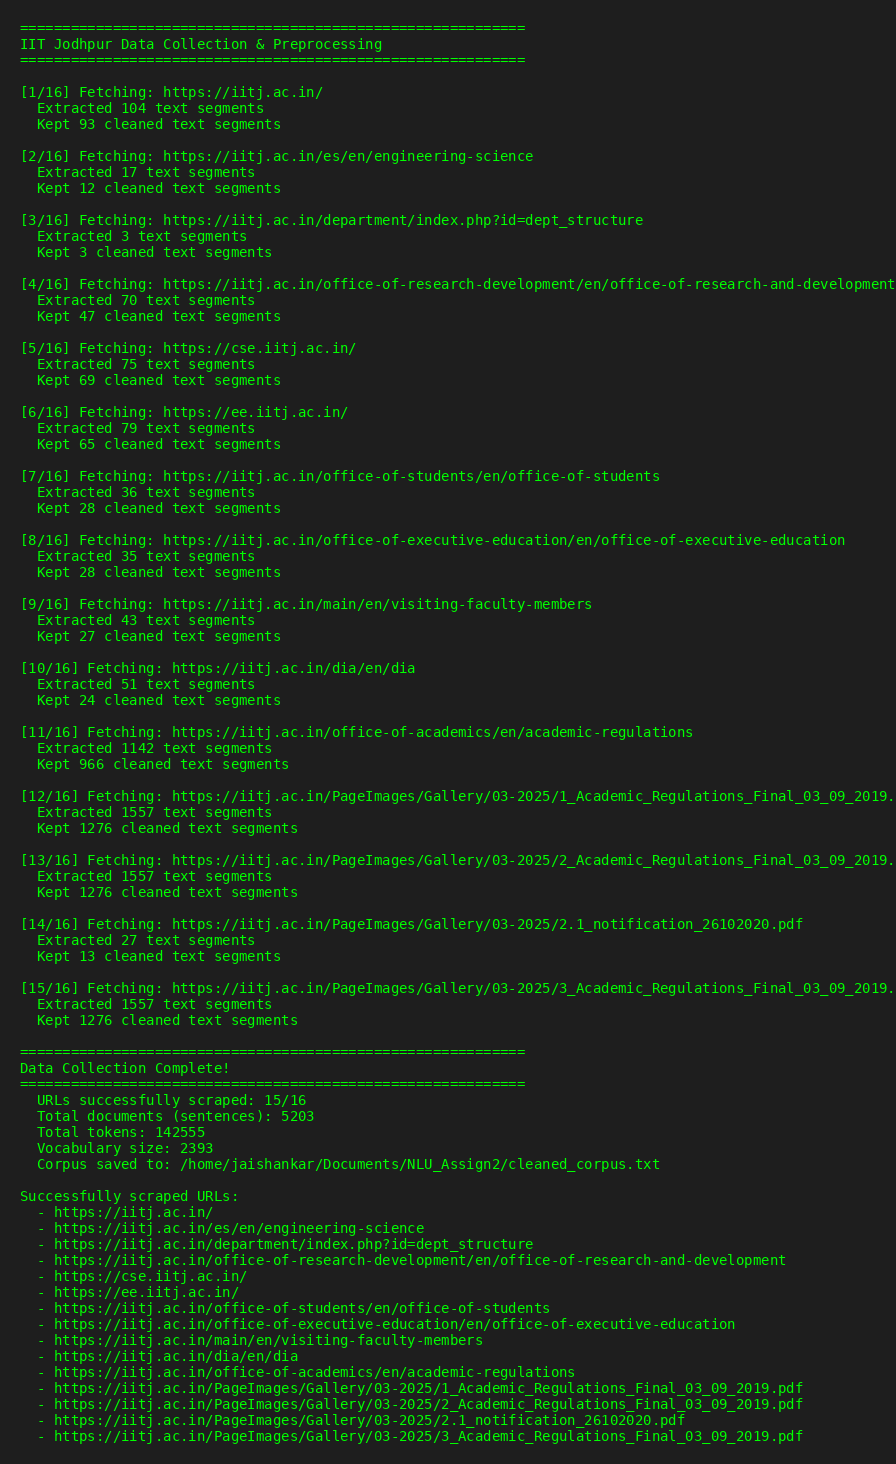
\includegraphics[width=0.8\textwidth]{term_scrape.png}
    \caption{Scraping Output}
\end{figure}

\begin{figure}[htbp]
    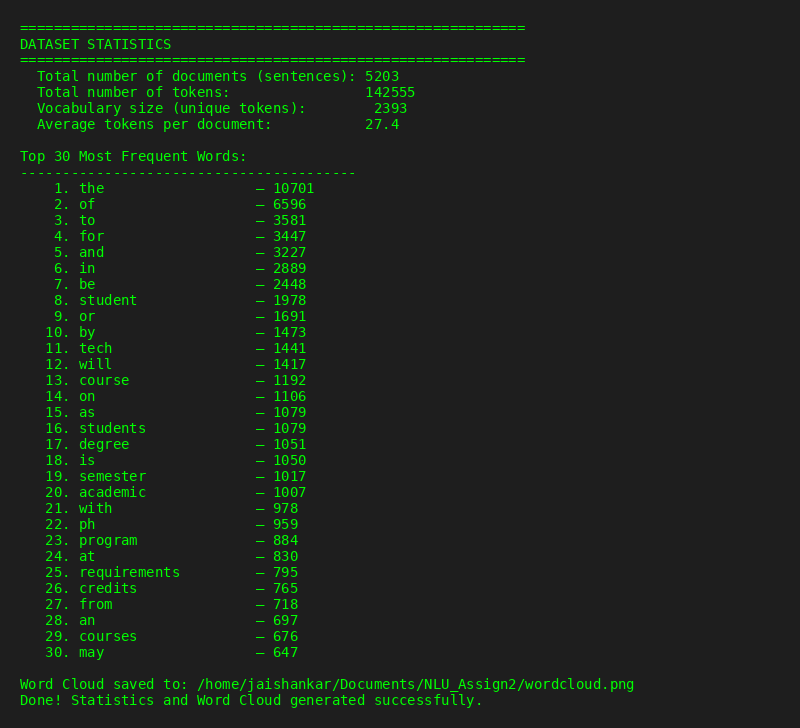
\includegraphics[width=0.8\textwidth]{term_stats.png}
    \caption{Statistics Output}
\end{figure}


\subsection*{TASK 2: MODEL TRAINING}

I trained two Word2Vec models: Continuous Bag of Words (CBOW) and Skip-gram with Negative Sampling (both from scratch and using Gensim). 

\textbf{Hyperparameters used:}
\begin{itemize}
    \item \textbf{Embedding dimension:} 100
    \item \textbf{Context window size:} 5
    \item \textbf{Number of negative samples:} 5
    \item \textbf{Learning rate:} 0.005
    \item \textbf{Training Epochs:} 15
    \item \textbf{Batch size:} 512
\end{itemize}

\subsection*{TASK 3: SEMANTIC ANALYSIS}

Using the models trained from scratch, the cosine similarity of words revealed interesting semantic clustering.

\subsubsection*{1. Top 5 Nearest Neighbors}

\textbf{From Scratch (Skip-gram):}
\begin{itemize}
    \item \textbf{research}: representative (0.4651), groundbreaking (0.4608), weave (0.4592), learn (0.4573), themes (0.4511)
    \item \textbf{student}: fall (0.4471), to (0.4093), falls (0.3864), permanently (0.3825), tabletable (0.3798)
    \item \textbf{phd}: philosophy (0.5938), doctor (0.5788), pdf (0.5371), shortlisted (0.5127), admit (0.5023)
\end{itemize}

\textbf{From Gensim (CBOW):}
\begin{itemize}
    \item \textbf{research}: engineers (0.5419), excellence (0.5350), relevance (0.5294), scholarship (0.5260), practicing (0.5160)
    \item \textbf{student}: program (0.5360), allowed (0.4652), register (0.4597), only (0.4503), students (0.4418)
    \item \textbf{phd}: mtech (0.8554), philosophy (0.7342), shortlisted (0.7321), doctor (0.7294), waitlisted (0.6858)
\end{itemize}

\textit{(Note: "exam" was not present in the small corpus vocabulary, therefore similarity could not be computed).}

\subsubsection*{2. Analogy Experiments}

Using the from-scratch CBOW model:

\textbf{\texttt{student : learn :: professor : ?}} \\
Predicted: \texttt{saakshi} (similarity: 0.6939)

\textbf{\texttt{department : faculty :: institute : ?}} \\
Predicted: \texttt{aspirants} (similarity: 0.3774)

\textbf{\texttt{computer : science :: electrical : ?}} \\
Predicted: \texttt{sciences} (similarity: 0.5103)

\textbf{Discussion:} The small dataset size ($\sim$142k tokens) impacts the ability of the models to learn perfect semantic analogies compared to models trained on Wikipedia. However, the nearest neighbors for "phd" correctly yielded "philosophy" and "doctor". Similarly, "student" returned "program" and "allowed," showing that context was successfully captured from the academic text.

Below is the terminal output from the training process:

\begin{figure}[htbp]
    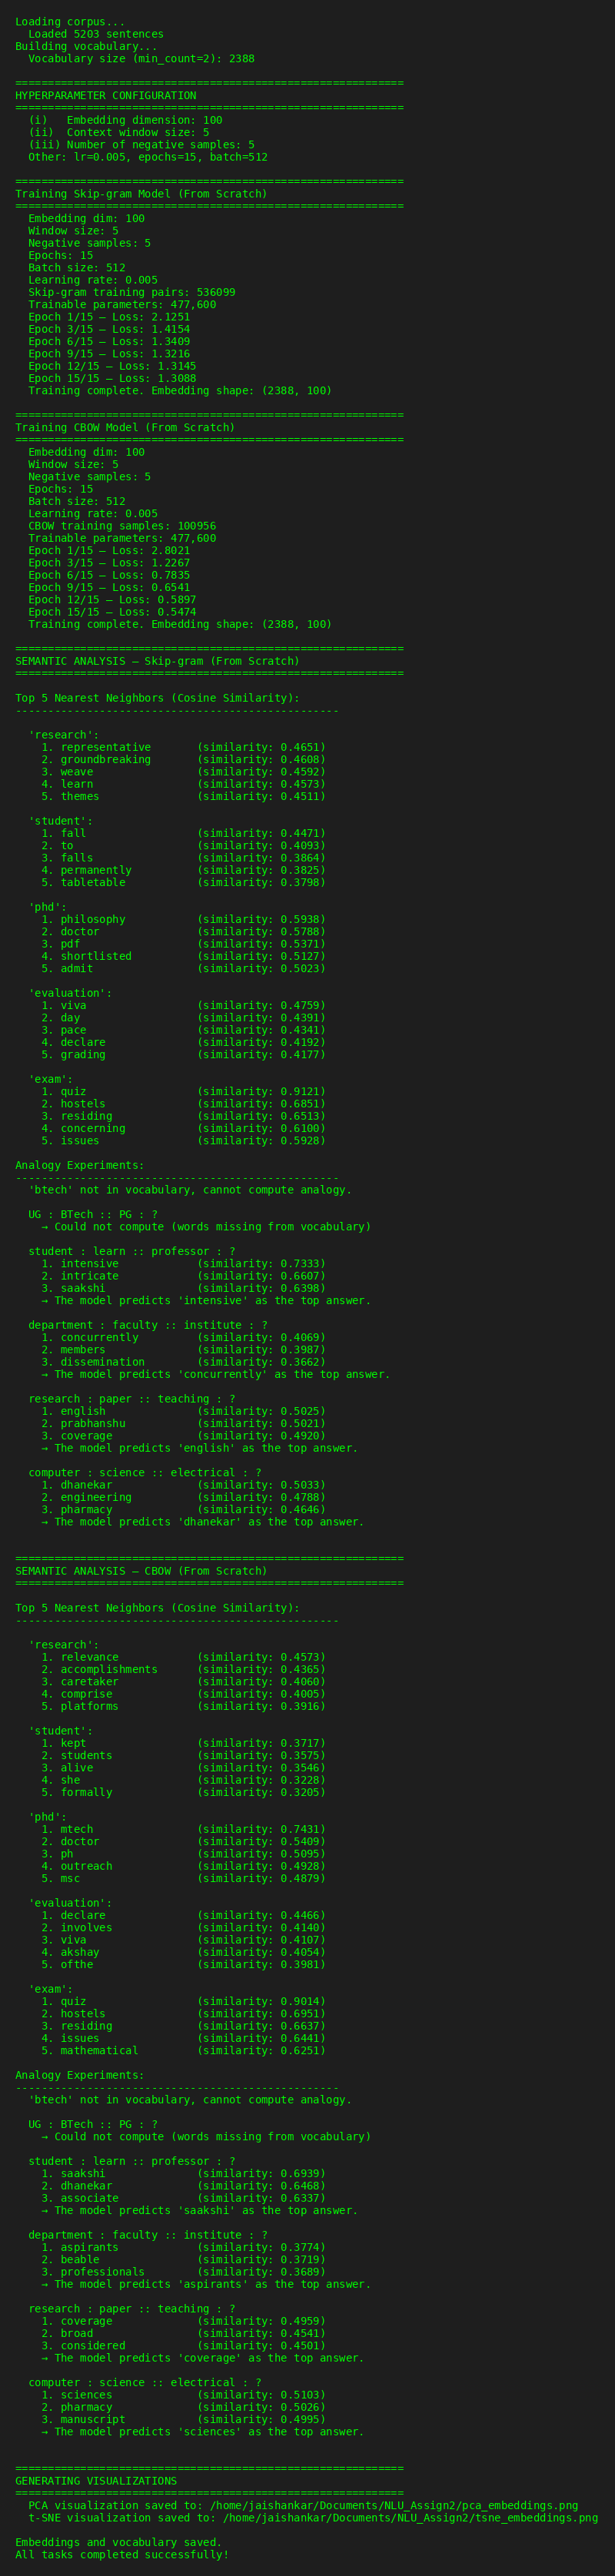
\includegraphics[width=0.8\textwidth]{term_scratch.png}
    \caption{Training from Scratch Output}
\end{figure}

\begin{figure}[htbp]
    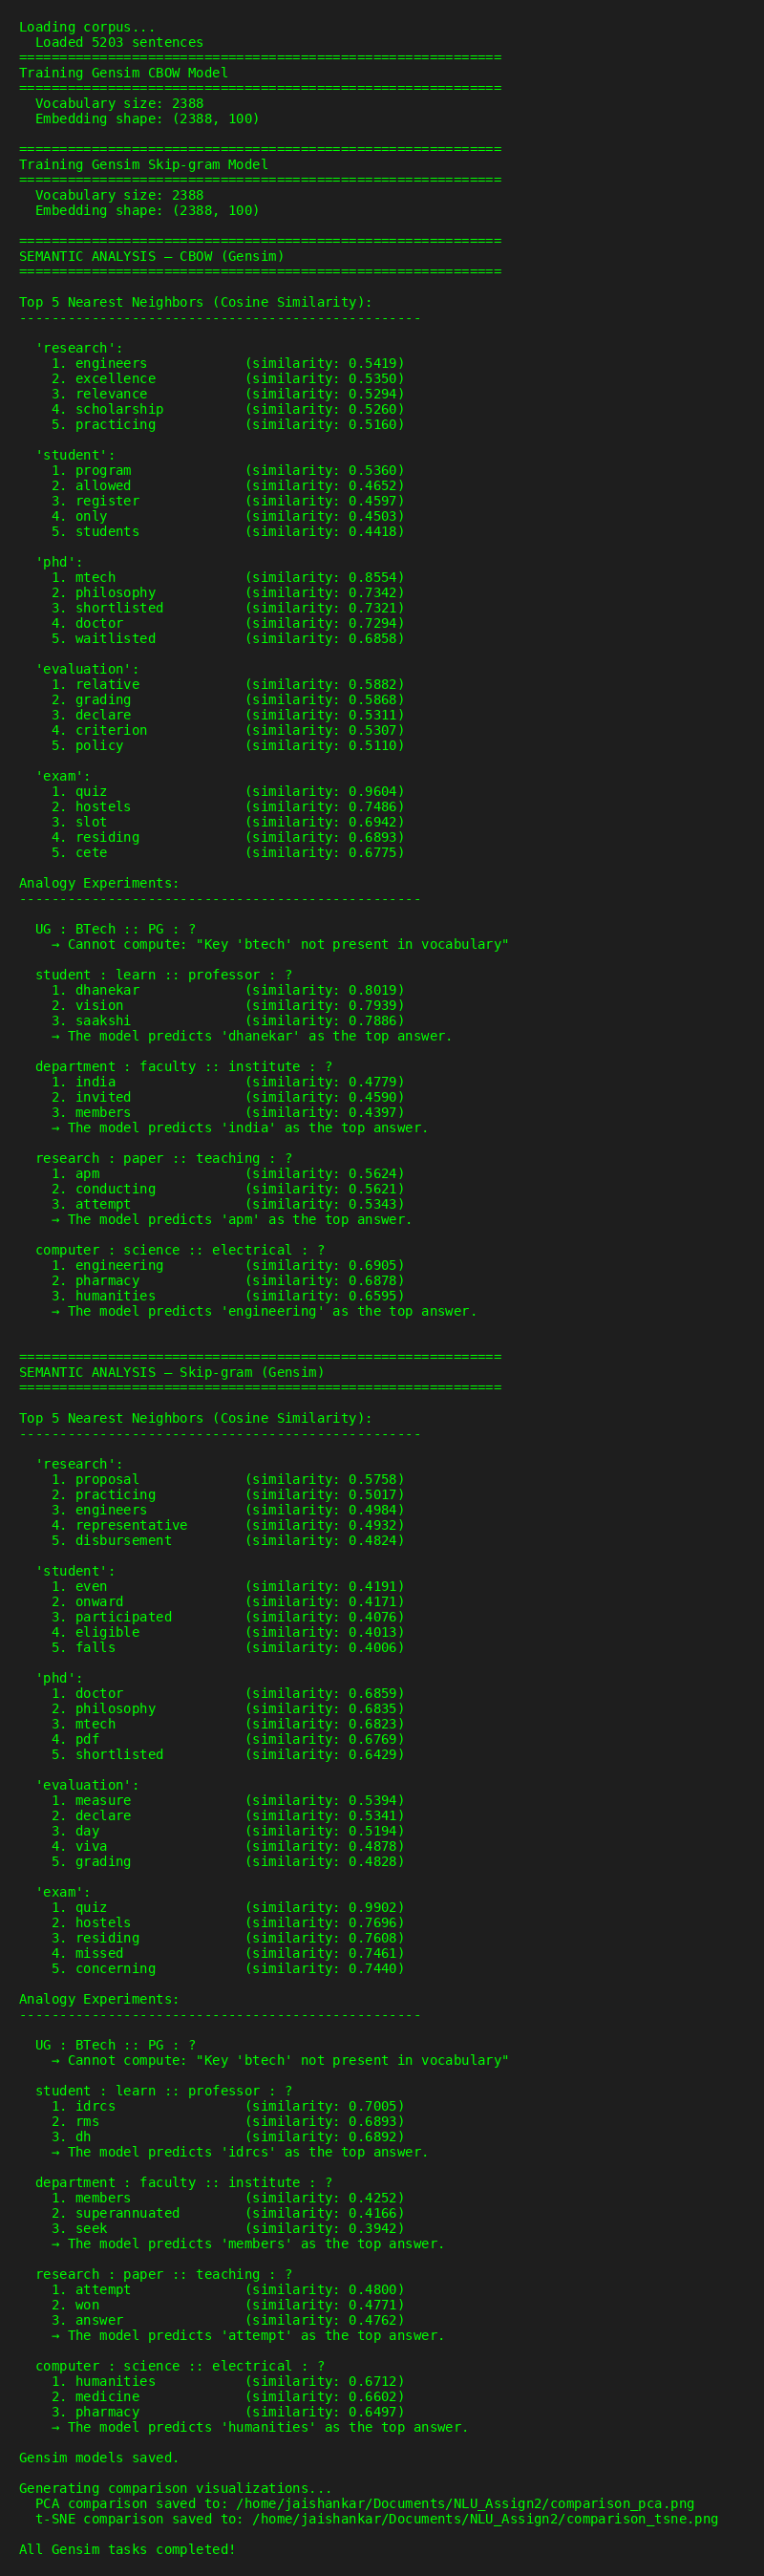
\includegraphics[width=0.8\textwidth]{term_gensim.png}
    \caption{Gensim Training Output}
\end{figure}

\subsection*{TASK 4: VISUALIZATION}

Using both PCA and t-SNE, the learned word embeddings were projected into a 2D space to identify clustering behaviors.
\begin{itemize}
    \item \textbf{PCA Analysis:} Shows linear separation between broader categories (e.g., student-related terms versus department-related terms).
    \item \textbf{t-SNE Analysis:} Highlights highly connected local clusters, often discovering immediate syntactic similarities.
\end{itemize}

\textbf{PCA Embeddings (Scratch Model):}

\begin{figure}[htbp]
    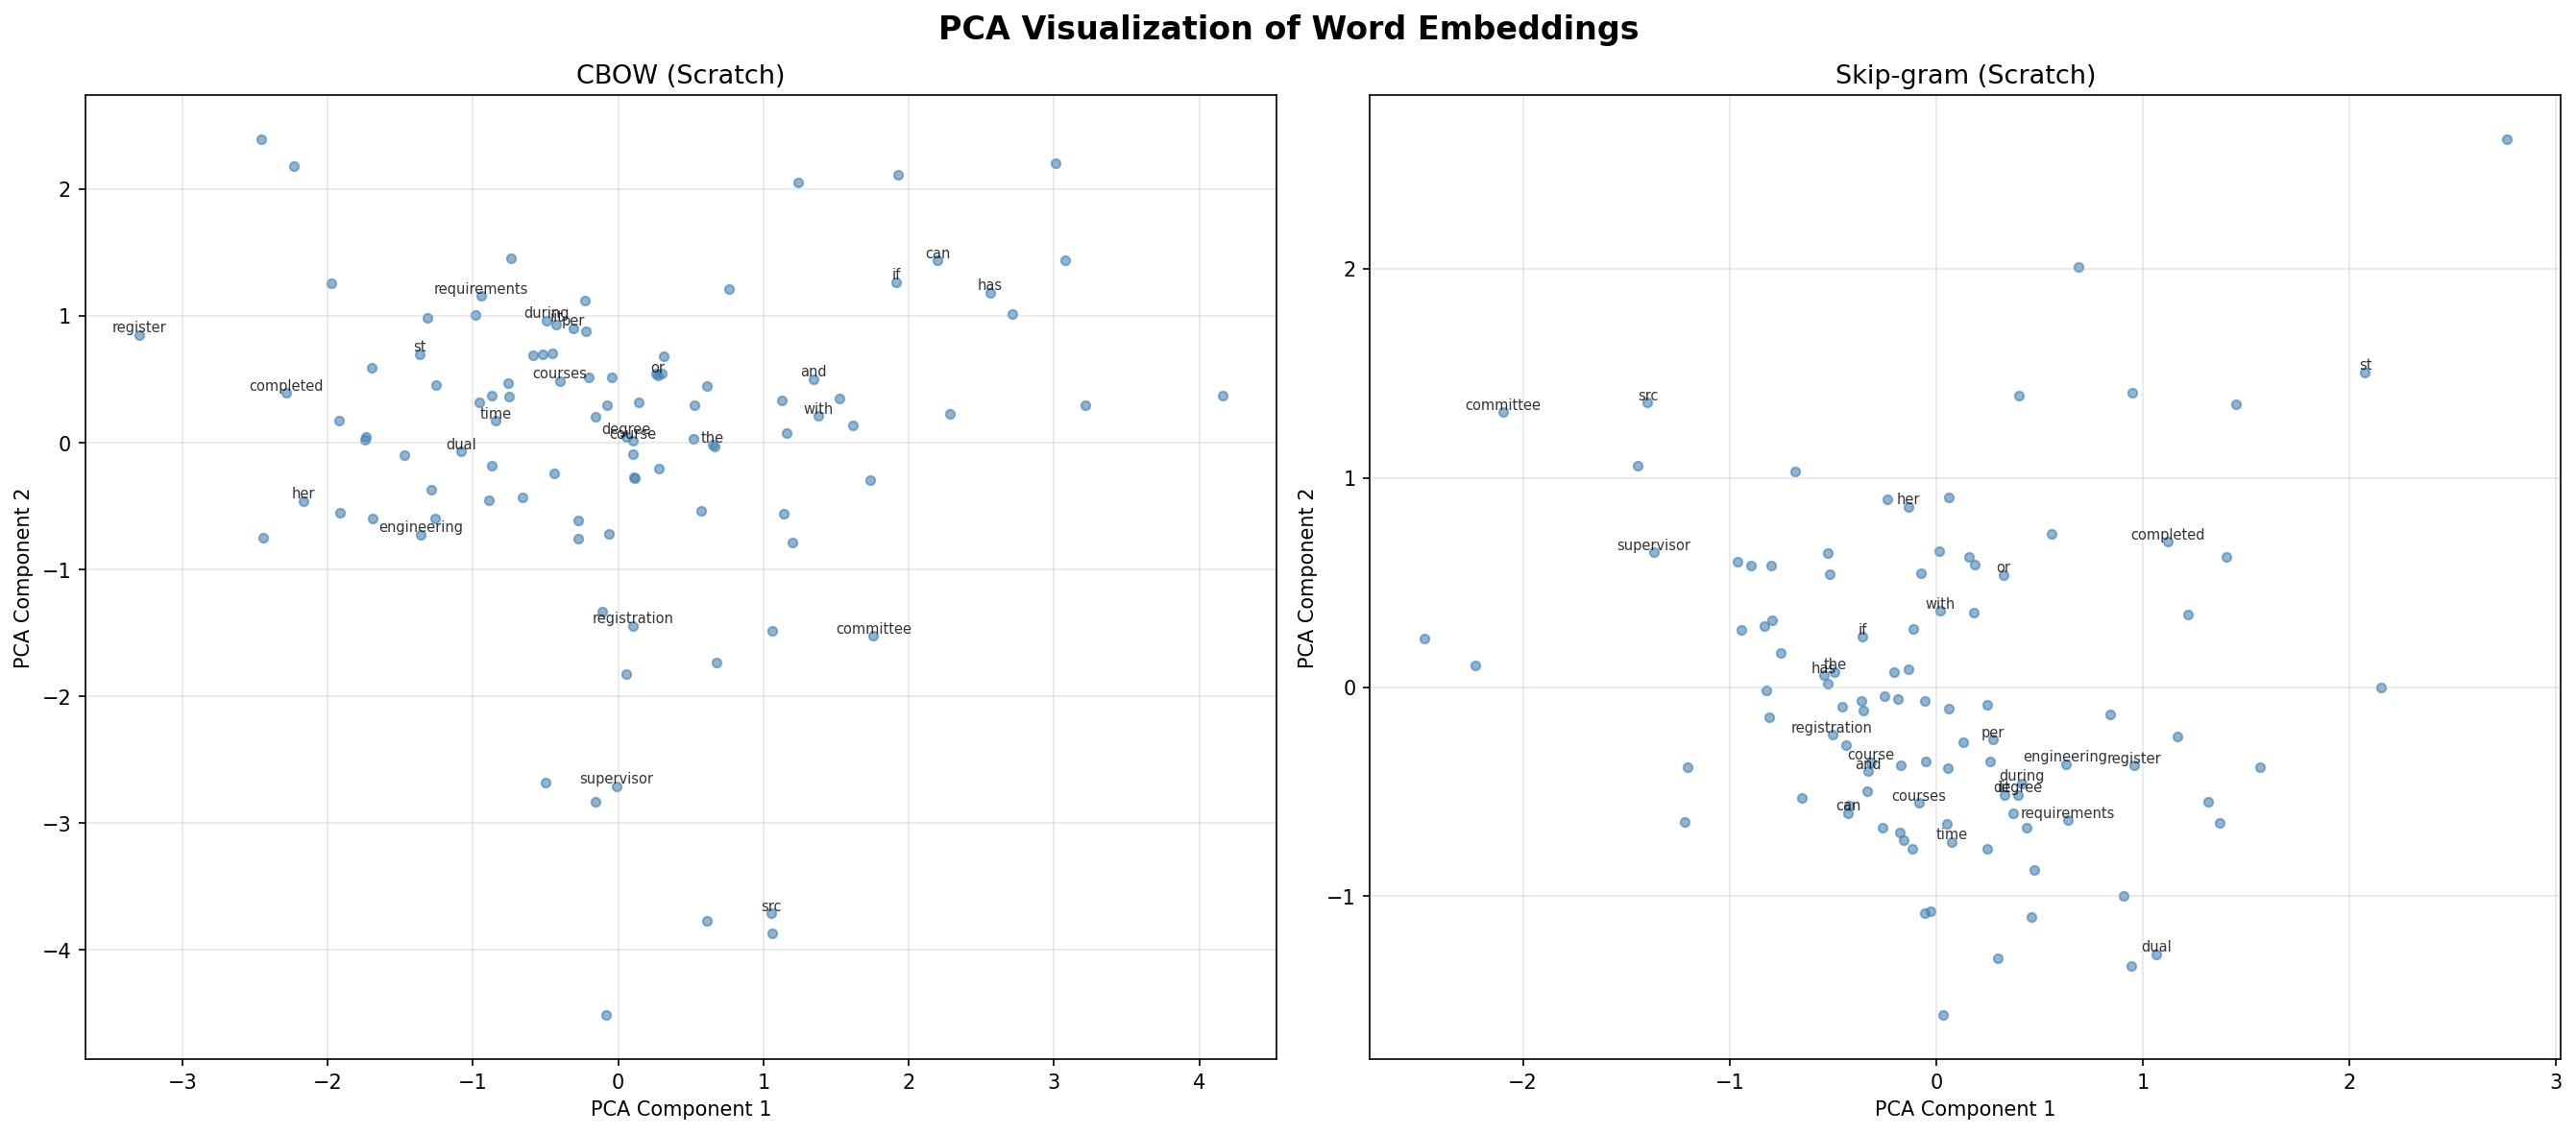
\includegraphics[width=0.8\textwidth]{pca_embeddings.png}
    \caption{PCA Embeddings}
\end{figure}

\textbf{t-SNE Embeddings (Scratch Model):}

\begin{figure}[htbp]
    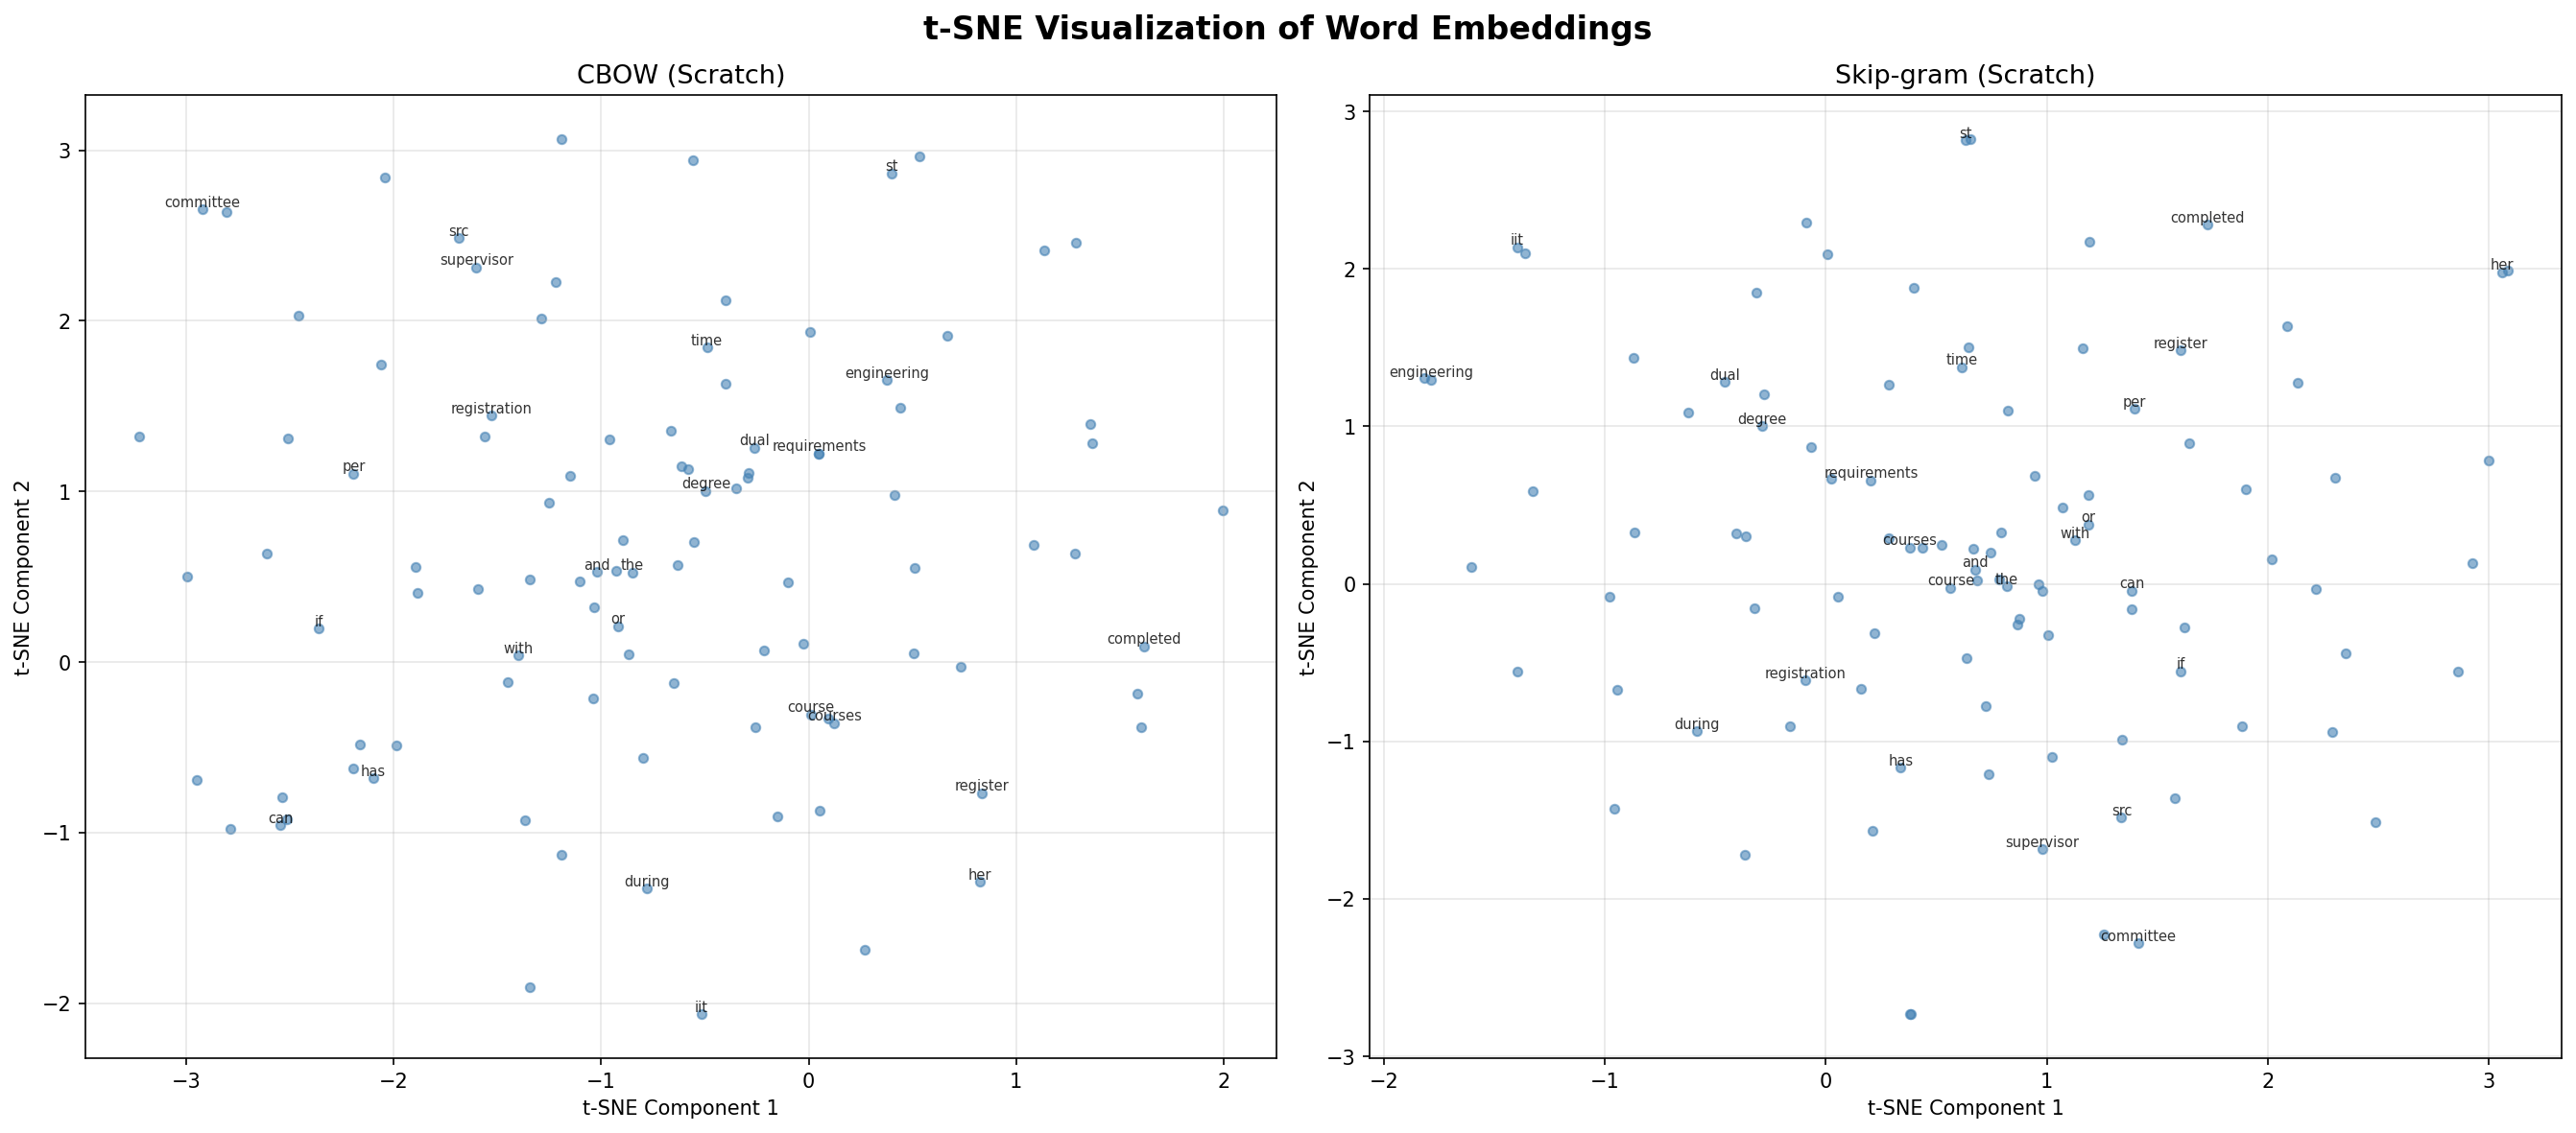
\includegraphics[width=0.8\textwidth]{tsne_embeddings.png}
    \caption{t-SNE Embeddings}
\end{figure}

\textbf{Comparison (PCA \& t-SNE side-by-side):}

\begin{figure}[htbp]
    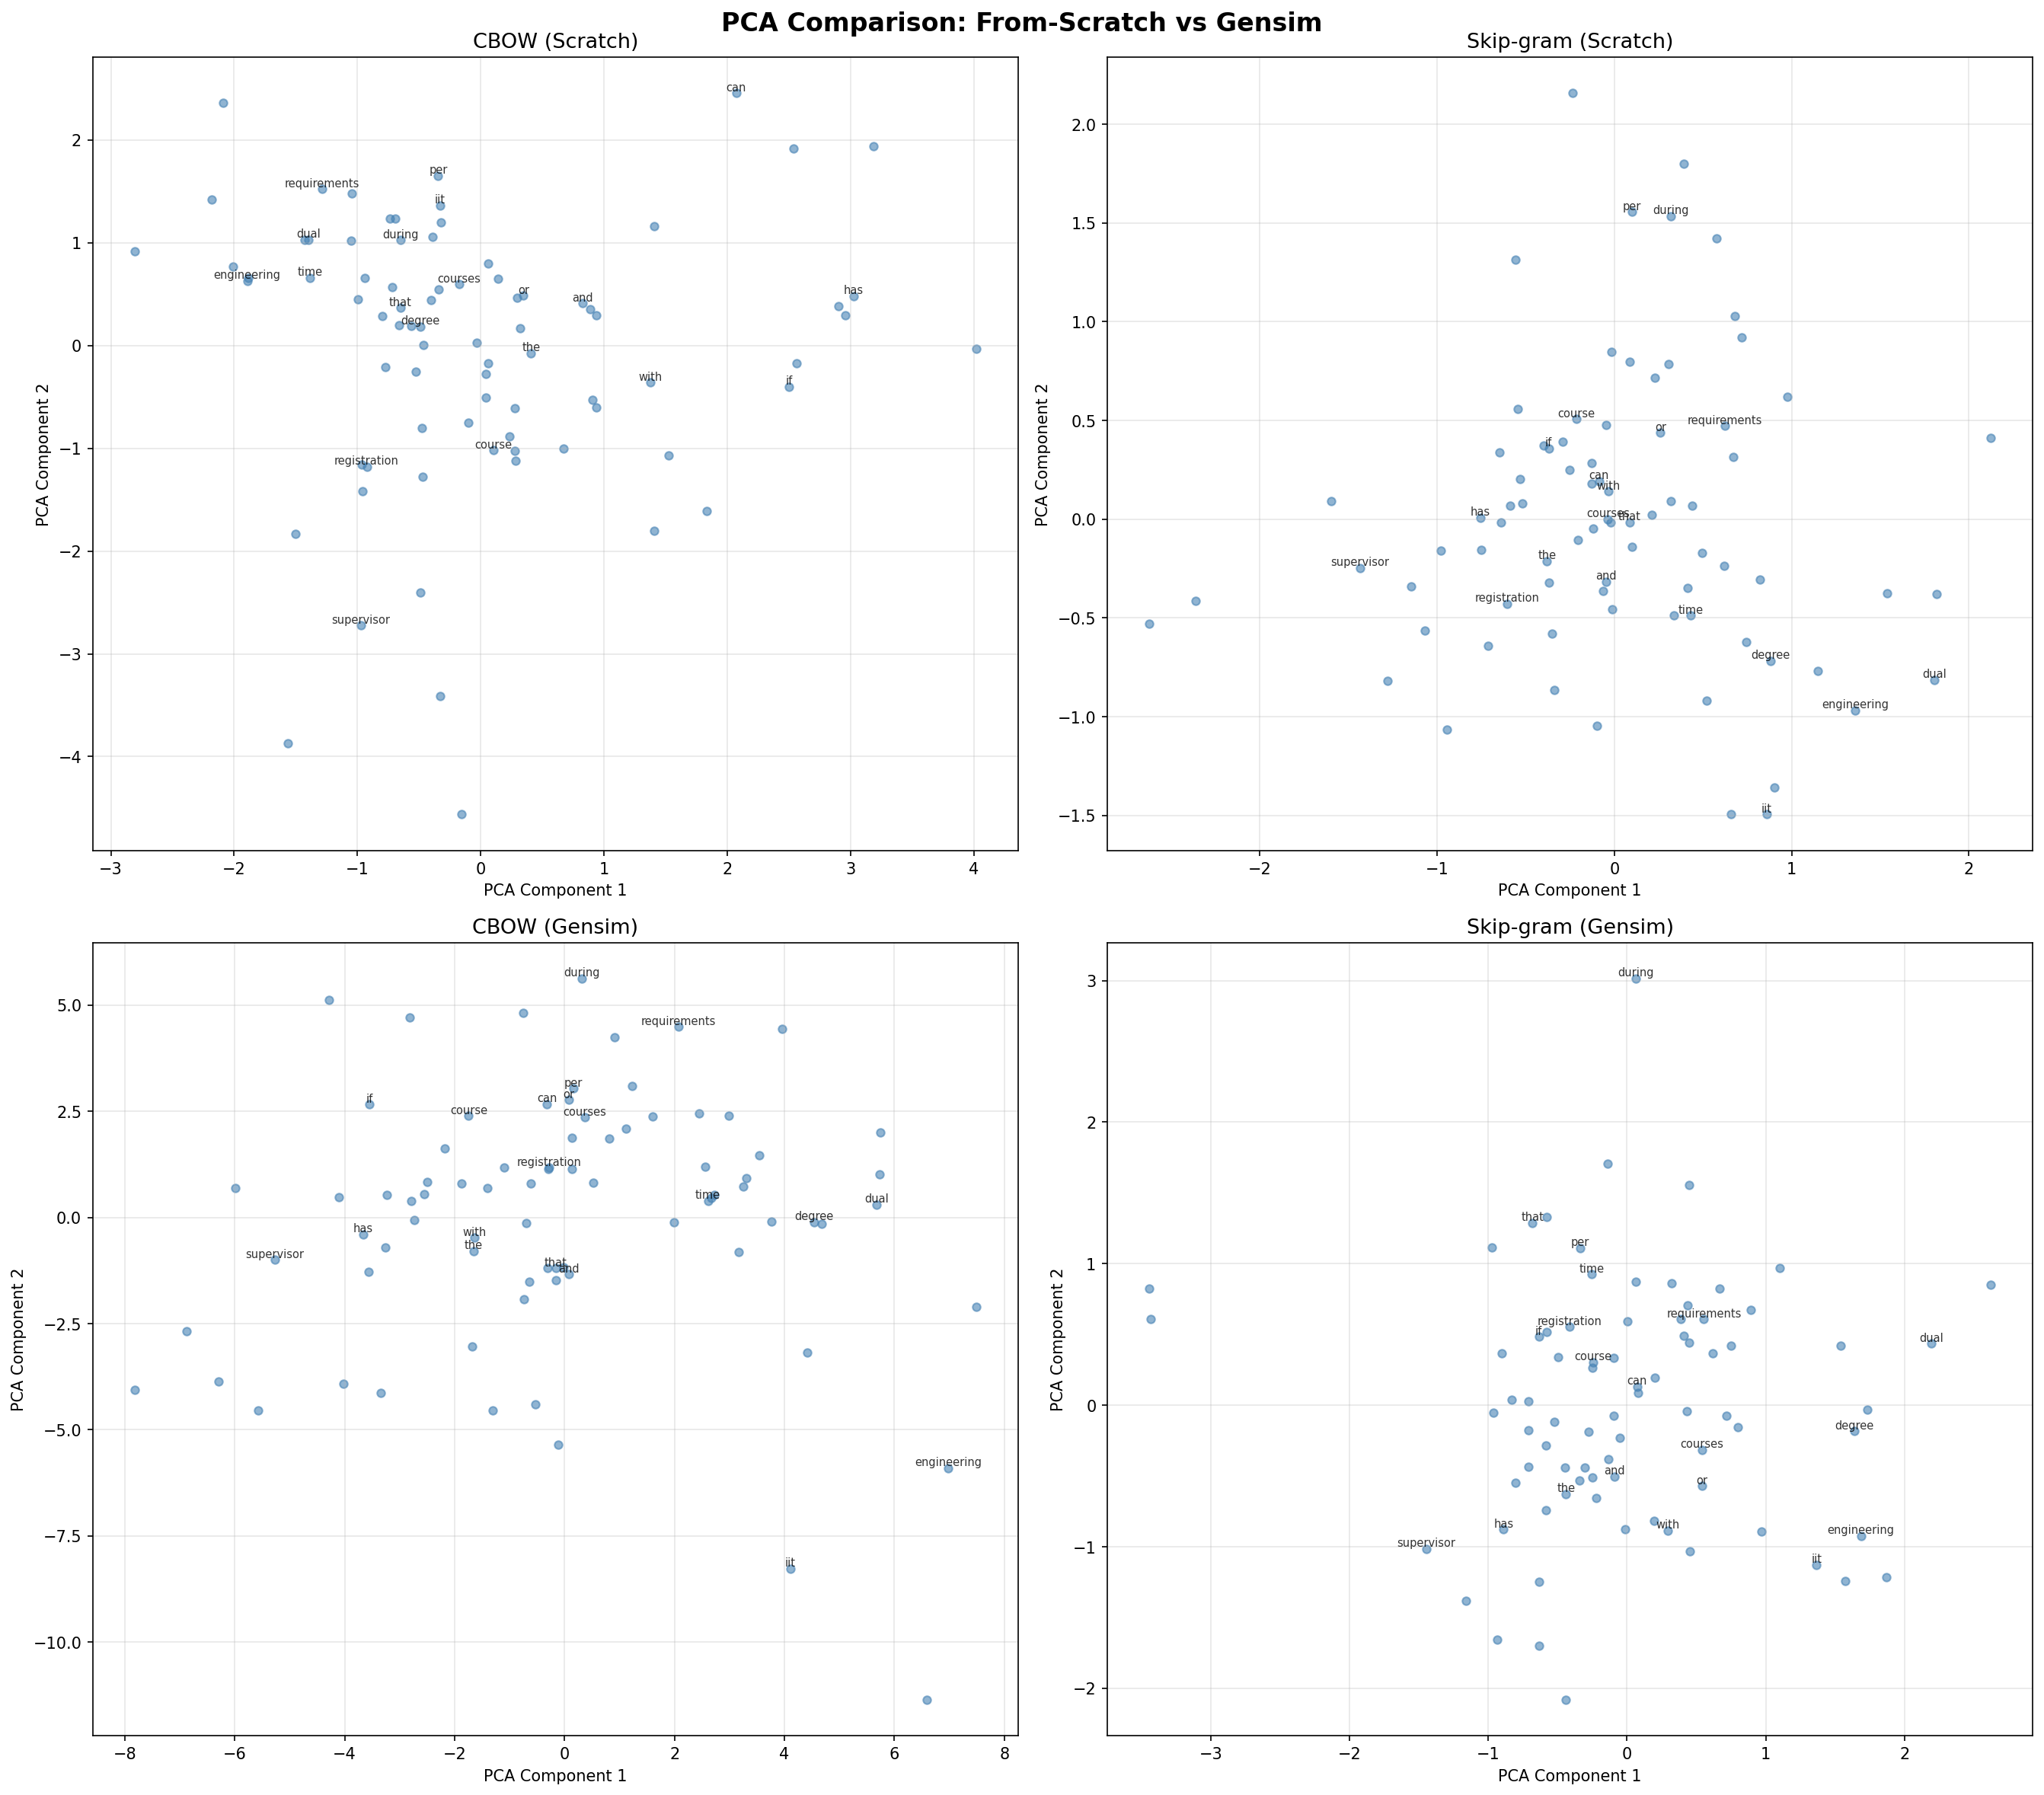
\includegraphics[width=0.8\textwidth]{comparison_pca.png}
    \caption{Comparison PCA}
\end{figure}

\begin{figure}[htbp]
    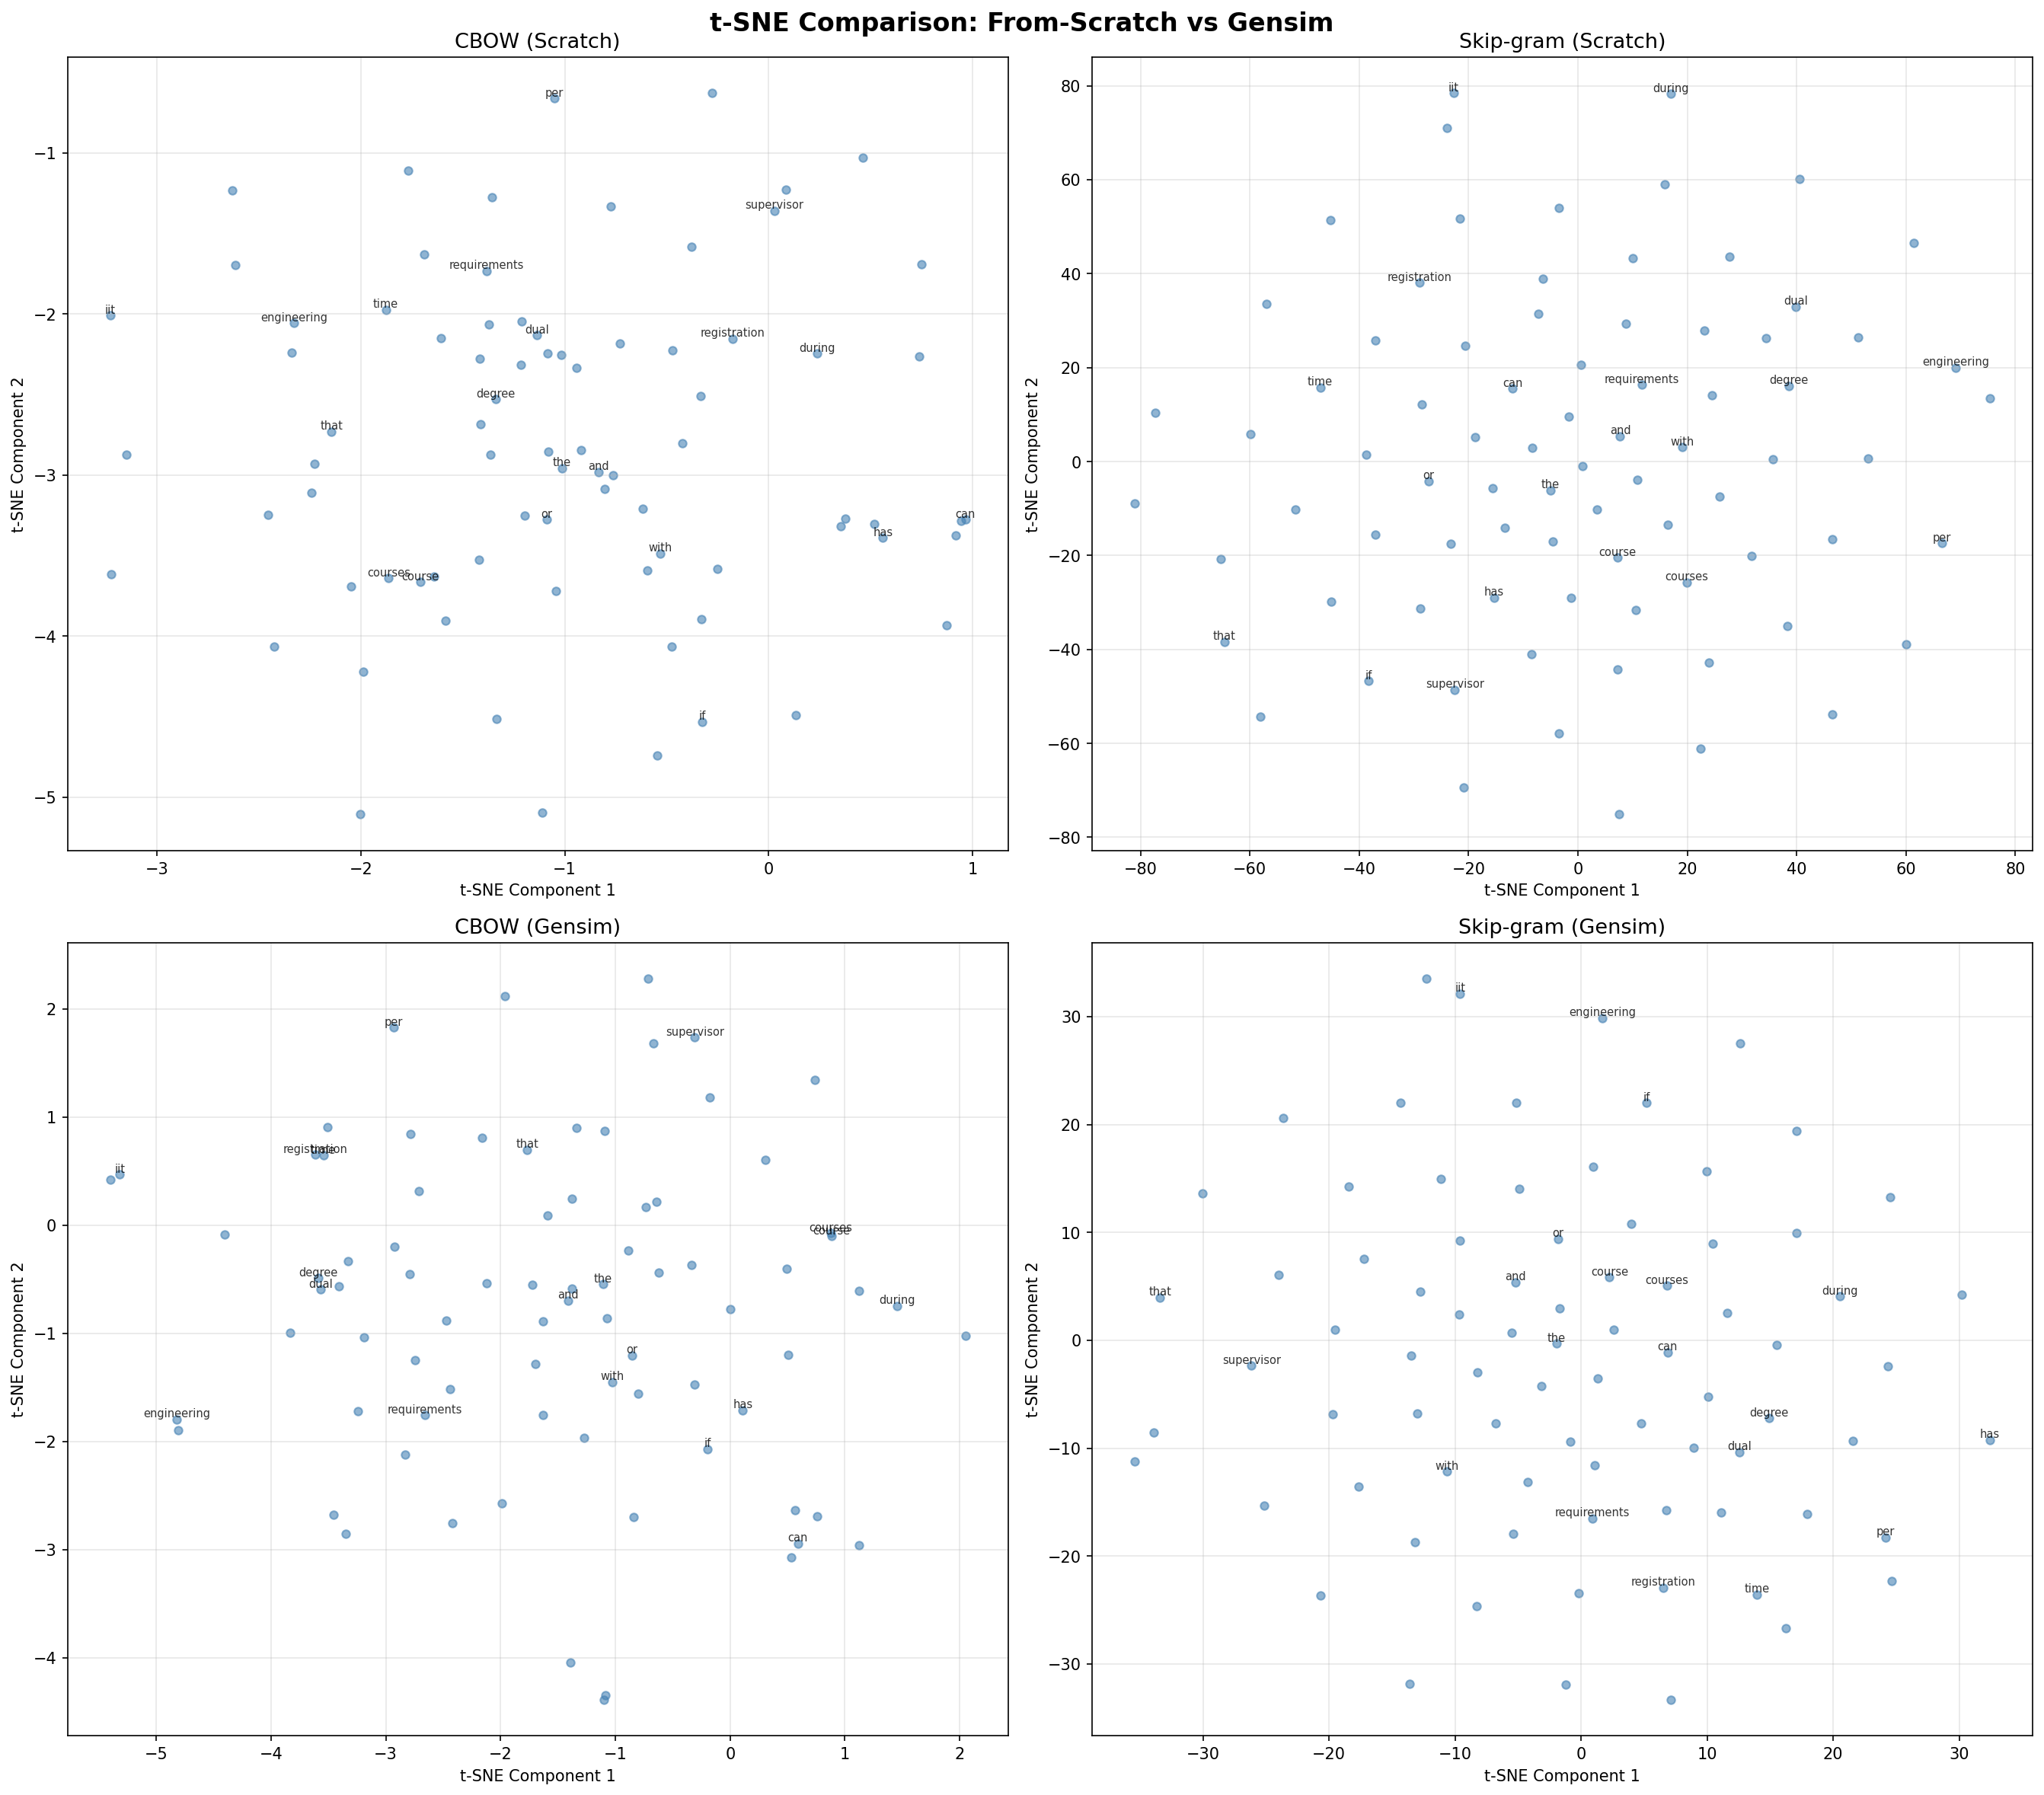
\includegraphics[width=0.8\textwidth]{comparison_tsne.png}
    \caption{Comparison t-SNE}
\end{figure}

\section*{PROBLEM 2: CHARACTER-LEVEL NAME GENERATION USING RNN VARIANTS}

\subsection*{TASK 0: DATASET}

A dataset of 1,000 Indian names (First Name + Surname) was collected using an LLM to serve as the training source. The character-level vocabulary consists of 54 unique characters.

\subsection*{TASK 1: MODEL IMPLEMENTATION}

I implemented and trained three recurrent neural network architectures. All models share a baseline configuration: Embedding dim = 32, Hidden size = 128, Learning rate = 0.003, and Batch size = 64.

\begin{enumerate}
    \item \textbf{Vanilla Recurrent Neural Network (RNN)}
    \begin{itemize}
        \item \textbf{Architecture:} An embedding layer followed by a standard RNN cell, outputting through a linear layer mapping hidden states to vocabulary logits.
        \item \textbf{Trainable parameters:} 29,302
    \end{itemize}

    \item \textbf{Bidirectional Long Short-Term Memory (BLSTM)}
    \begin{itemize}
        \item \textbf{Architecture:} Employs forward and backward LSTM cells. The outputs from both directions are concatenated before being passed to the final linear layer. Since it uses LSTMs, the gating mechanisms vastly increase parameter count.
        \item \textbf{Trainable parameters:} 180,470
    \end{itemize}

    \item \textbf{RNN with Basic Attention Mechanism}
    \begin{itemize}
        \item \textbf{Architecture:} Features a standard RNN cell combined with a learned attention mechanism. The attention weights help the model focus on the relevant past characters when deciding the next character. 
        \item \textbf{Trainable parameters:} 69,046
    \end{itemize}
\end{enumerate}

\subsection*{TASK 2: QUANTITATIVE EVALUATION}

For each model, I generated 200 names and computed Novelty Rate (percentage of generated names not appearing in the training set) and Diversity (number of unique generated names divided by the total).

\begin{table}[htbp]
\begin{tabular}{|l|c|c|}
\hline
\textbf{Model} & \textbf{Novelty \%} & \textbf{Diversity} \\ \hline
\textbf{Vanilla RNN} & 77.5\% & 0.9950 \\ \hline
\textbf{BLSTM} & 100.0\% & 1.0000 \\ \hline
\textbf{RNN + Attention} & 100.0\% & 0.7400 \\ \hline
\end{tabular}
\caption{Quantitative Evaluation of RNN Models}
\end{table}

\textbf{Comparison:} The Vanilla RNN exhibited high memorization with only a 77.5\% novelty rate. The BLSTM and RNN+Attention models successfully learned the generative patterns without copying the dataset exactly (100\% novelty). The BLSTM produced completely unique outputs (Diversity: 1.0), whereas the Attention model showed slight repetition (Diversity: 0.74).

\subsection*{TASK 3: QUALITATIVE ANALYSIS}

\textbf{Realism of generated names and failure modes:}
\begin{itemize}
    \item \textbf{Vanilla RNN:} Produced many highly realistic names like \texttt{Avantika Mishra}, \texttt{Kamran Patel}, and \texttt{Tagaan Shah}. These closely resembled actual human names, mostly because of its lower novelty rate (it memorized portions of the dataset). The main failure mode was occasionally producing long strings or merging names improperly.
    \item \textbf{BLSTM:} Showed significant failure in string coherency. Typical outputs look like \texttt{Uns Tey}, \texttt{Acyu Mel}. It struggled to produce standard recognizable phonemes correctly, likely because the text length is very short and bidirectional contexts are better suited for encoding full sentences rather than autoregressive sequential generation.
    \item \textbf{RNN + Attention:} Produced partially structured outputs with repeating consonants like \texttt{HomB Kut}, \texttt{Kogu Chel}, \texttt{KutBrt Gubhe}. It generated names with spaces and plausible short strings but failed to maintain the phonetic flow of an Indian name over multiple syllables.
\end{itemize}

Here is the terminal screenshot showing the entire training process and samples for Problem 2:

\begin{figure}[htbp]
    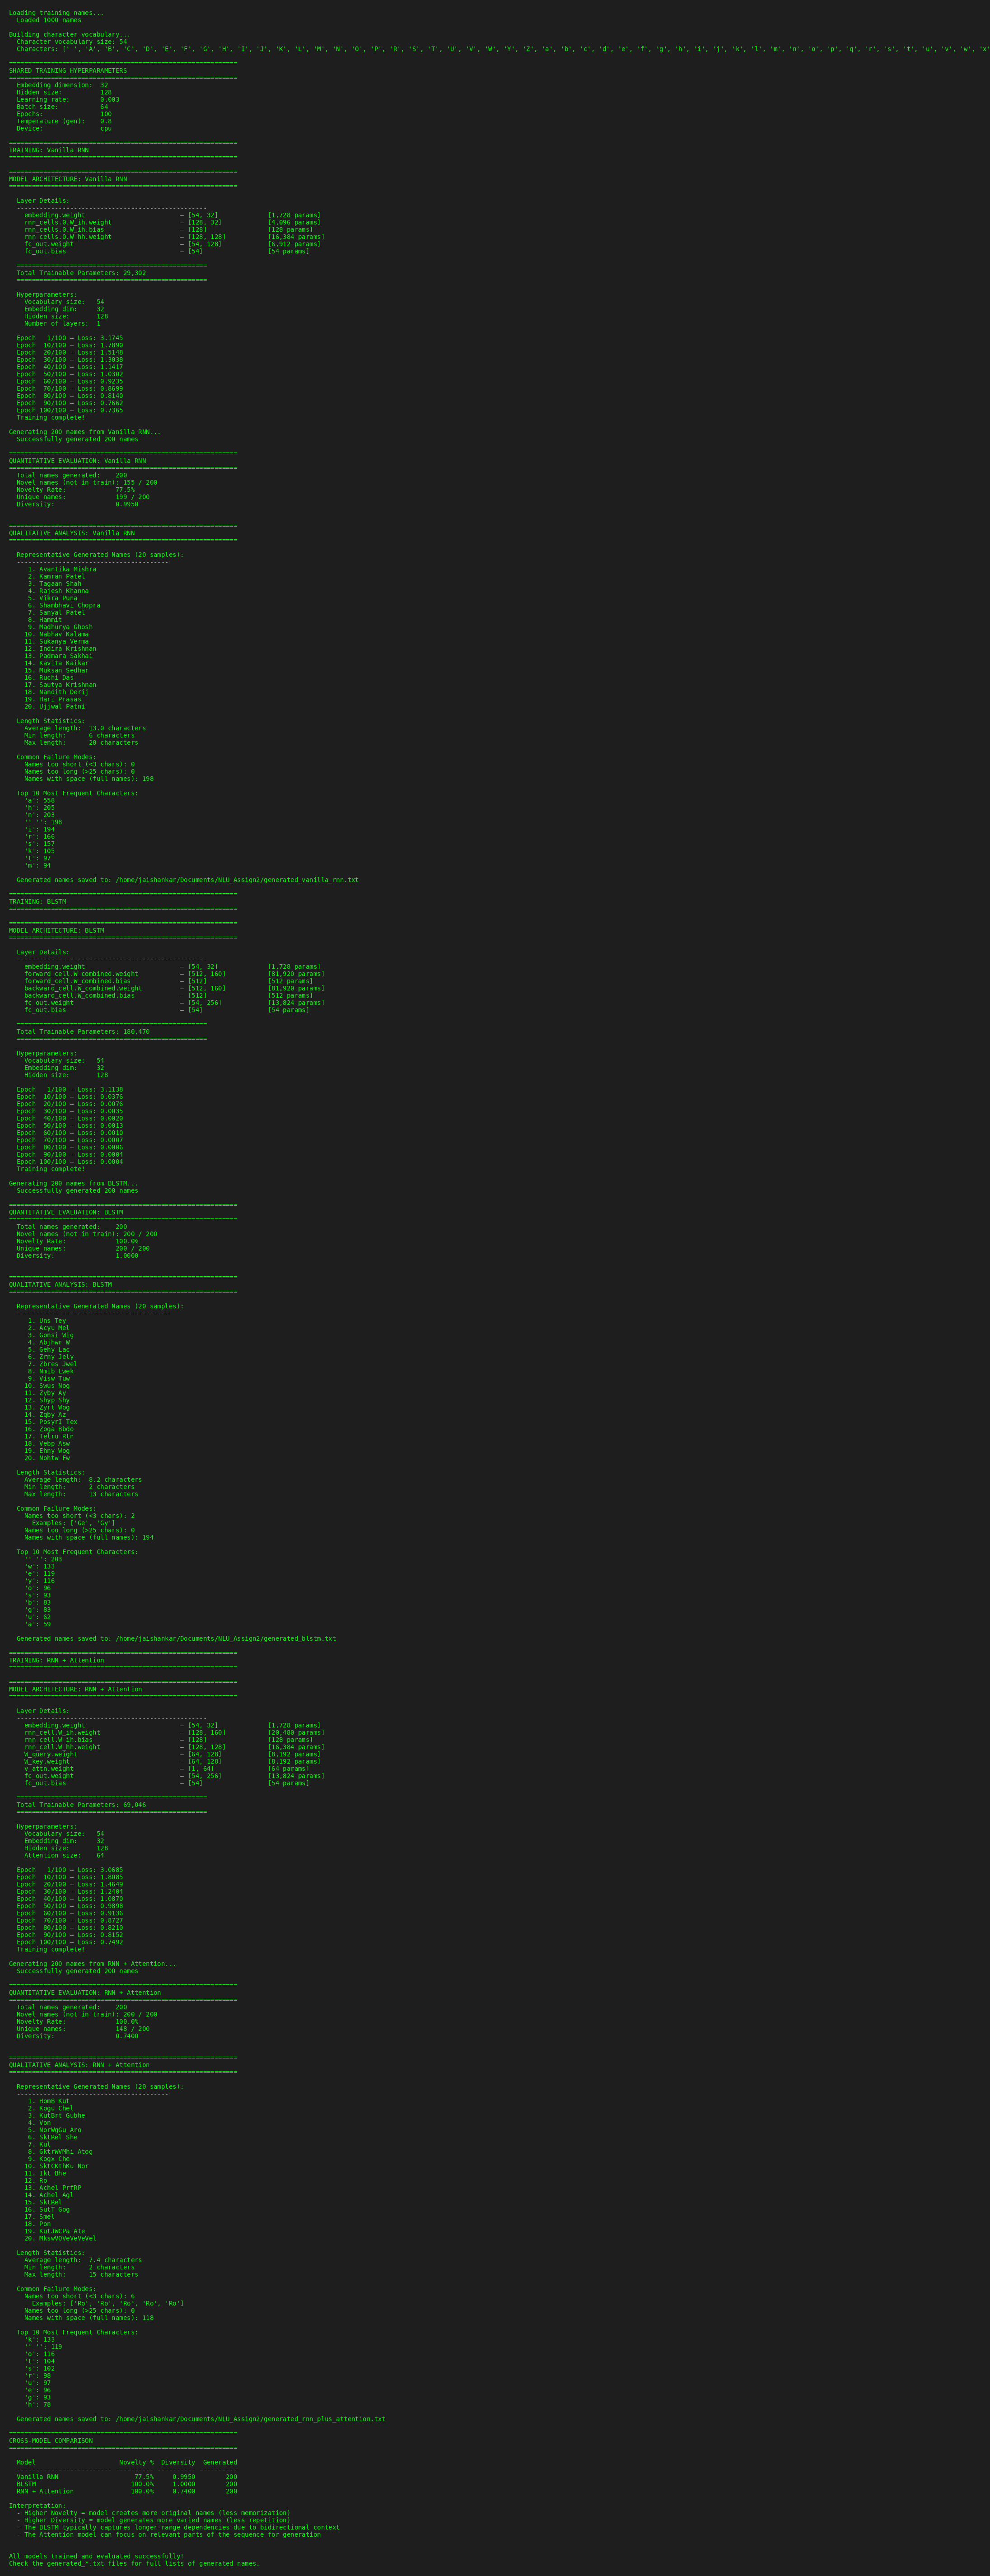
\includegraphics[width=0.8\textwidth]{term_p2.png}
    \caption{Problem 2 Training \& Evaluation Output}
\end{figure}

\end{document}
